\pgfplotsset{
    axis lines=middle,
    axis line style={->},
    xmin=0,
    xmax=4.2*pi,
    xticklabels=empty,
    xtick=\empty,
    ymin=-1,
    ymax=1,
    yticklabels=empty,
    ytick=\empty,
    samples=200,
    domain=0:4*pi,
    every axis plot post/.append style={very thick},
    clip=false
}% end of common axis set
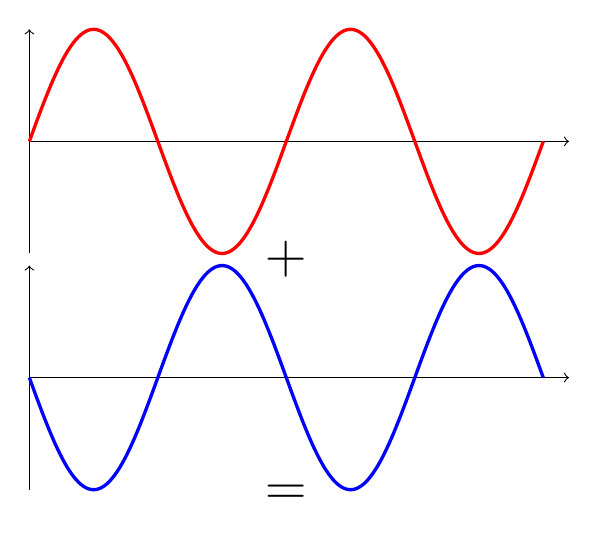
\begin{tikzpicture}
    \begin{axis}% 1. plot
        [yscale=0.5]
        \addplot[red] {(sin(deg(x)))};
        \node at (2*pi,-1.05) {\huge$+$};
    \end{axis}
    \begin{axis}% 2. plot
        [ yshift=-3cm,yscale=0.5]
        \addplot[blue] {(sin(deg(x+pi)))};
        \node at (2*pi,-1.05) {\huge$=$};
    \end{axis}
\end{tikzpicture}

\begin{tikzpicture}
    \begin{axis}% 3. plot
        \addplot[purple] {0};
    \end{axis}
\end{tikzpicture}
